    \subsection{Algoritmo de simplificación por proximidad de objetos}

    % Autoridad > derecho limitado a una porcion
    % Claridad > autoridad no ambigua
    % Anticipacion > avisar con antelacion
    % Granularidad > rutas cortas y funcionales
    % Terminalidad > avisar fin de via
    % Infraestructura > avisar de infraestructura
    % No bloqueo > circulacion fluida
    
    Todos los algoritmos de generación de señalamiento explicados en la Sección \ref{sec:generacion} colocan el señalamiento a una distancia fija, que llamaremos X, del elemento que buscan proteger. Existe, por lo tanto, una región espacial del tendido ferroviario anterior y posterior al elemento ferroviario donde se situarán las señales, que denominaremos región de señalamiento. 
    
    Si la distancia entre dos elementos ferroviarios es menor a 2X pero mayor a X, las señales generadas para proteger la región de señalamiento que comparten ocupará el mismo espacio físico. En este caso, el principio anticipación no se cumple porque las señales correspondientes se entremezclan, no dando suficiente tiempo para informar al conductor que un nuevo elemento ferroviario se encuentra delante. Incluso las señales podrían alterar su orden en esta región, avisando primero del próximo elemento antes de anunciar la partida del elemento que se está transitando en ese momento.

    Si la distancia entre dos elementos ferroviarios es menor a X, las señales generadas para proteger la región de señalamiento que comparten ocupará el espacio físico correspondiente al otro elemento. Esto repercute negativamente en la claridad de las autoridades otorgadas a los conductores, impidiendo que se cumpla el principio de claridad. Tampoco se cumpliría el principio de anticipación y de no bloqueo, al no avisar con antelación la existencia de los peligros ni permitiría una circulación fluida al detener la marcha en el medio de otro elemento.

    El RNA aplica el Algoritmo \ref{alg:proximity} para solucionar este inconveniente, analizando los objetos cercanos de a pares. Cuando la distancia entre dos objetos es menor a un parámetro dado, las señales son movidas. Las señales de advertencia, previas a un elemento ferroviario, son anticipadas, salteando el elemento que provoca el solapamiento de señales. Las señales de partida son retrasadas, mas allá del elemento que provoca el solapamiento de señales. El resultado obtenido es que ambos elementos ferroviarios, al situarse tan próximo uno del otro, se consideran prácticamente como un solo elemento ferroviario a proteger.

    \begin{algorithm}[hbt!]
        \caption{Algoritmo de simplificación por proximidad de objetos}
        \label{alg:proximity}
        \DontPrintSemicolon
        %\SetAlgoLined
        \SetNoFillComment
        \LinesNotNumbered 
            Given \{Signals\},\{objects\}\\
            \For {object\_A in objects}
            {
                \For {object\_B in objects}
                {
                    \If {object\_A != object\_B}
                    {
                        \If {dist(object\_A,object\_B) $<$ MIN\_DISTANCE}
                        {
                            move\_signals\_between(\{Signals\},object\_A,object\_B)
                        }
                    }
                }
            }
            \KwResult{\{Signals\}} 
    \end{algorithm}
    
    La Figura \ref{fig:signal_proximity} ilustra un sistema de vía simple con un paso a nivel (Lc01) y una plataforma (Plat01) para tres casos: suficiente separación entre elementos (vía superior), poca distancia entre los elementos sin aplicar el Algoritmo \ref{alg:proximity} (vía intermedia) y poca distancia entre elementos pero aplicando el Algoritmo \ref{alg:proximity} (vía inferior).
    
    \begin{figure}[h!]
        \centering
        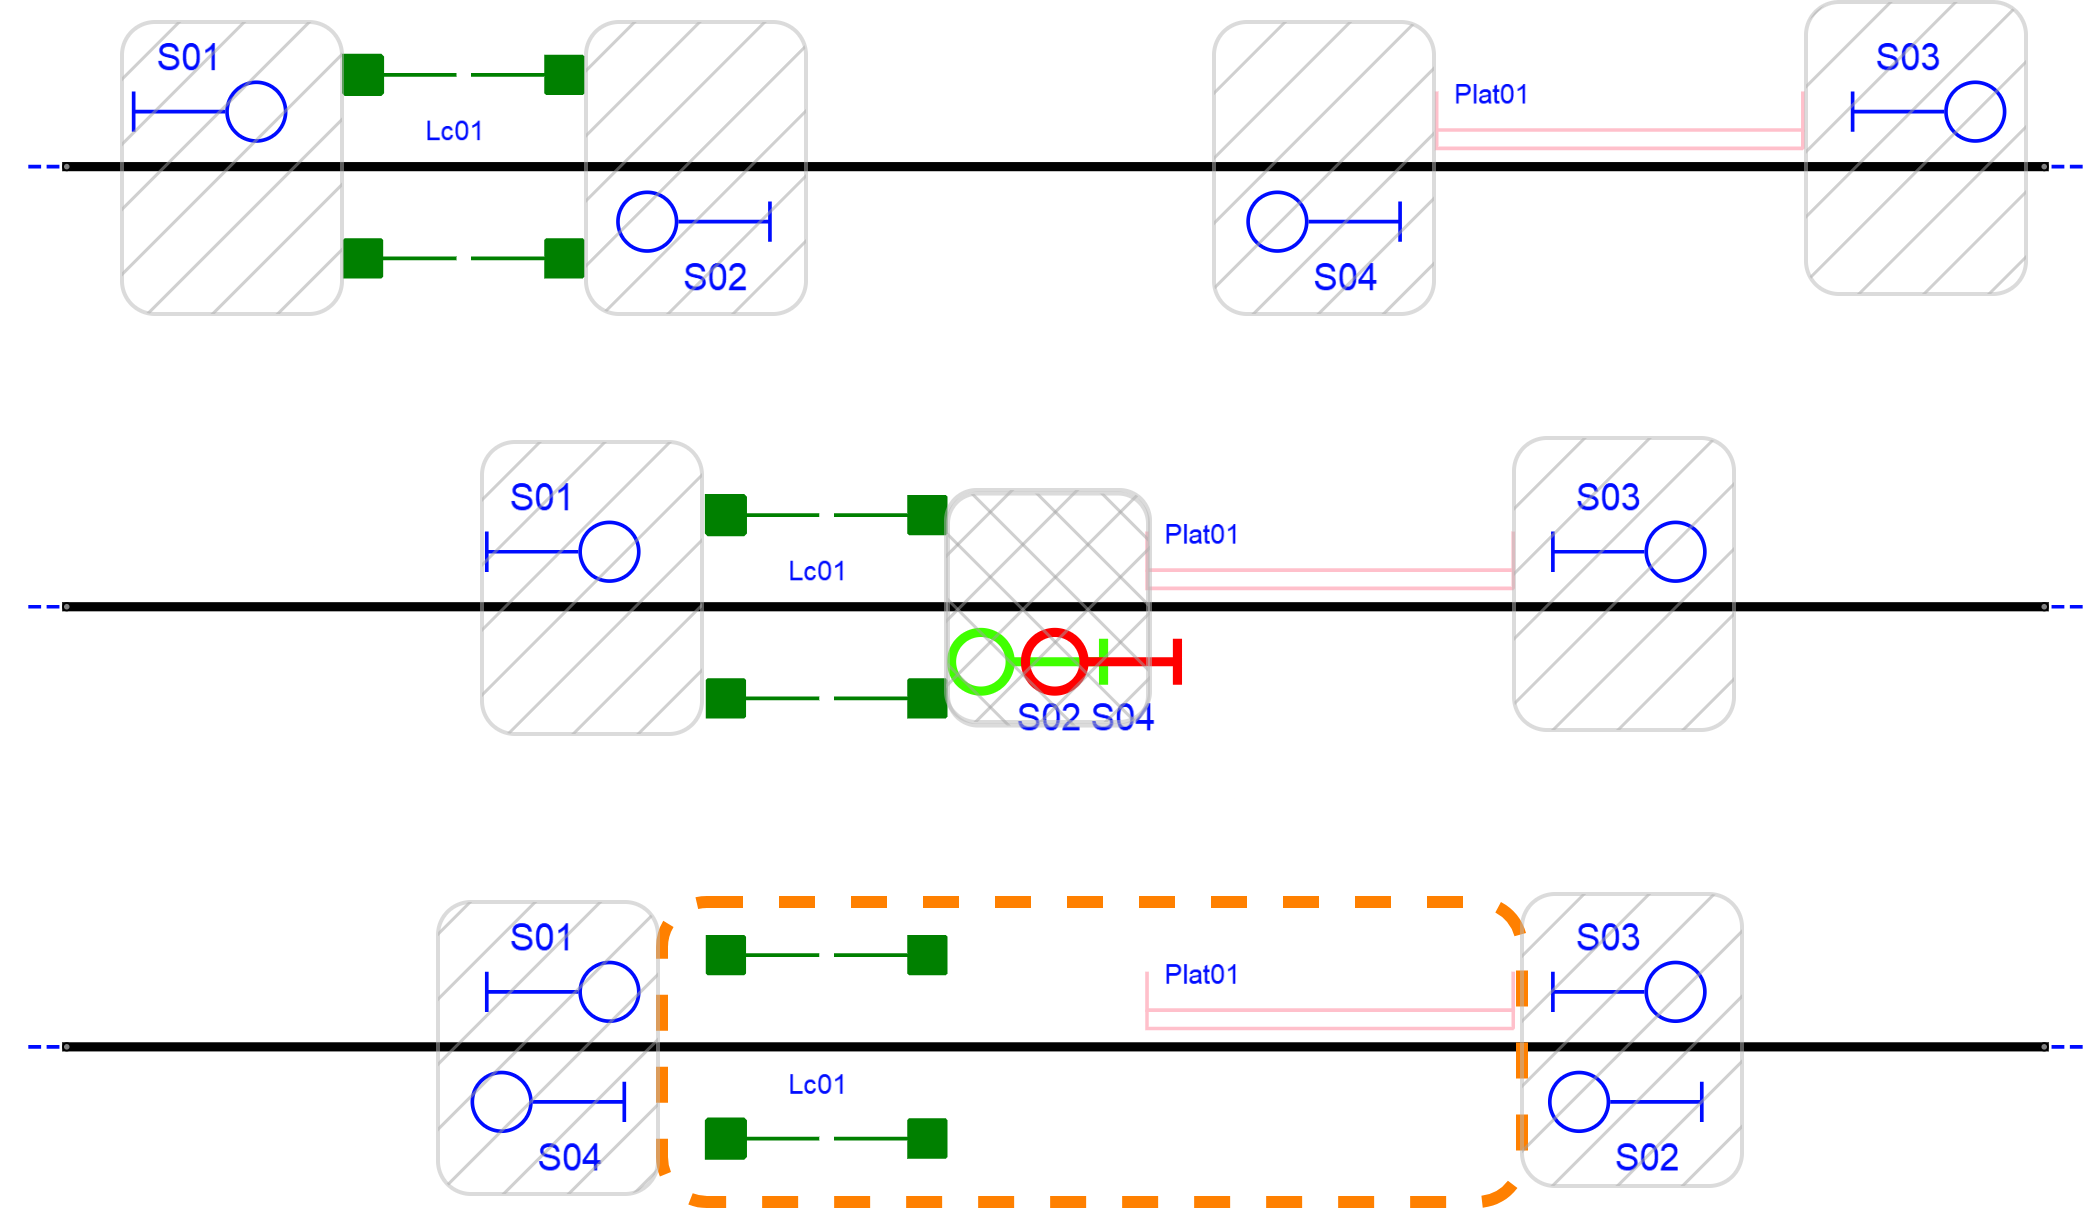
\includegraphics[width=1\textwidth]{Figuras/proximity.PNG}
        \centering\caption{Simplificación del señalamiento generado por proximidad de objetos.}
        \label{fig:signal_proximity}
    \end{figure}

    En la vía superior se presenta el caso de un paso a nivel y una plataforma separados una distancia suficiente. Esta distancia es tal que sus regiones de señalamiento (indicadas mediante rayas grises oblicuas) no se solapan. Por lo tanto, las señales S01 y S02 que protegen el paso a nivel y las señales de partida de la plataforma S03 y S04 no interfieren entre si.

    En la vía intermedia, la distancia entre ambos elementos ferroviarios fue reducida. Las regiones de señalamiento entre el paso a nivel y la plataforma se solapan. En función de los parámetros de distancia al paso a nivel y la plataforma elegidos para el señalamiento, las señales S02 y S04 pueden estar en distinto orden. Es decir, una formación que circula de derecha a izquierda podría ver primero la señal S02 y luego la señal S04, o viceversa, en base a los parámetros de configuración elegidos. Incluso la señal S02 podría situarse sobre la plataforma y la señal S04 dentro del paso a nivel. Todos casos no deseados, que alteran el funcionamiento normal de la red y van en contra de los principios de señalamiento.

    En la vía inferior tenemos la misma infraestructura que en la vía intermedia, pero se aplicó el Algoritmo \ref{alg:proximity}. La señal S02 que se utilizaba para detener la formación previo a un paso a nivel en caso de que la barrera aún no estuviese baja es adelantada al comienzo de la plataforma. De esta manera, el conductor se detendrá algunos metros antes del paso a nivel. La señal S04 que se utilizaba como señal de partida de la plataforma es retrasada hasta después del paso a nivel. De esta manera, la formación partida de la plataforma cuando el aspecto de la señal S04 sea verde, pero eso no sucederá en tanto y en cuanto la barrera del paso a nivel no se encuentre baja.

    La aplicación del Algoritmo \ref{alg:proximity} despeja las señales que quedaron atrapadas en el poco espacio físico entre ambos elementos ferroviarios. El resultado final es la anulación de la región de señalamiento intermedia, considerando a la entidad Lc01-Plat01 como un mismo elemento ferroviario, resaltado en el recuadro naranja de la Figura \ref{fig:signal_proximity}. Este nuevo elemento adopta las funcionalidades de ambos elementos individuales simultáneamente: la formación debe detenerse en la plataforma hasta que la señal de partida habilite su salida y solo se podrá atravesar el paso a nivel si la señal de circulación lo habilita previa confirmación de que la barrera se encuentra baja.

    El Algoritmo de simplificación por proximidad de objetos puede aplicarse a mas elementos, combinándolos en entidades mas grandes de ser necesario. El señalamiento resultante protegerá ambos extremos del nuevo elemento, sin sacrificar ninguna de las funcionalidades de sus miembros.